\chapter{Sensoren und Aktoren}
Zur Kommunikation mit dem technischen Prozess sind Sensoren und Aktoren, die eine physikalische Größe in eine Spannung/Strom (bzw. vice versa) umwandeln notwendig.
Um die Daten digital zu verabeiten ist zudem ein Analog-Digital-Umsetzer (ADC) sowie ein Digital-Analog-Umsetzer (DAC) notwendig.
Beim Auslegen des Eingebetteten Systems muss entschieden werden, in welchem Punkt die Digital-Analog-Wandlung stattfindet: entweder an den Sensoren/Aktoren, das
heißt die Daten werden dann digital übertragen oder an der CPU, das heißt die Signale werden dann analog übertragen.

\begin{table}[H]
    \centering
    \begin{tabular}{p{.5\textwidth}p{.5\textwidth}}
        \toprule
        ADC/DAC bei der CPU & ADC/DAC bei den Sensoren/Aktoren \\
        \midrule
        + Weniger Bauteile benötigt & + CPU-Modul weniger komplex \\
        + Höhere Integration & + Angepasster ADC/DAC möglich \\
        - Störanfällig & - Kommunikation nicht trivial \\
        - Analog-Prozess in Fertigung & \\
        \bottomrule
    \end{tabular}
    \caption{Vor und Nachteile für verschiedene Platzierung des ADC/DAC}
\end{table}

Es gibt Analoge Sensoren (z.B. Entfernung), sowie digital Sensoren (z.B. Lichtschranke).

\section{Grundbegriffe der Messtechnik}
\subsection{DIN-1316: Messen}
\paragraph{Messen} 
Ein experimenteller Vorgang, durch den eine physikalische Größe als Vielfaches einer Einheit oder eines Bezugswertes ermittelt wird.

\todo{Mehr im Moodle}

\paragraph{Messumformer} 
Ein analoges Eingangssignal wird in ein eindeutig damit zusammenhängendes analoges Außgangssignal unter der Aufbringung von Energie umgeformt (Verstärker).

\paragraph{Messwandler}
Messumformer, der die selbe physikalische Größe am Ein- und Ausgang aufweißt, und ohne externe Energie auskommt.

\paragraph{Messumsetzer}
Messgerät, das am Eingang und Ausgang verschiedene Signalstrukturen (Analog/Digital) aufweißt.

$\Rightarrow$ In ES sind Analog-Digital-Umwandler von besonderer Bedeutung.

\section{Analog-Digital-Umwandler}
\begin{figure}[H]
    \centering
    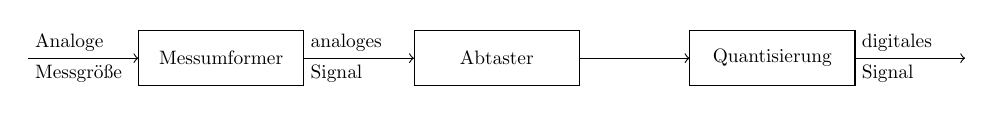
\begin{tikzpicture}[scale=0.7, every node/.style={scale=0.7}]
        \draw[->] (0,0.5) |- (2,0.5);
        \node [above right] at (0,0.5) {Analoge};
        \node [below right] at (0,0.5) {Messgröße};
        \filldraw [draw=black,fill=white] (2,0) rectangle (5,1);
        \node at (3.5,0.5) {Messumformer};
        \draw[->] (5,0.5) |- (7,0.5);
        \node [above right] at (5,0.5) {analoges};
        \node [below right] at (5,0.5) {Signal};
        \filldraw [draw=black,fill=white] (7,0) rectangle (10,1);
        \node at (8.5,0.5) {Abtaster};
        \draw[->] (10,0.5) |- (12,0.5);
        \filldraw [draw=black,fill=white] (12,0) rectangle (15,1);
        \node at (13.5,0.5) {Quantisierung};
        \draw[->] (15,0.5) |- (17,0.5);
        \node [above right] at (15,0.5) {digitales};
        \node [below right] at (15,0.5) {Signal};
    \end{tikzpicture}
    \caption{Aufbau eines ADUs}
\end{figure}

Es wird nach zwei Arten von Umsetzern unterschieden:
\begin{itemize}
    \item Zeitdiskrete-ADUs: Die Messgröße wird in regelmäßigen Abständen abgetastet und eine Probe der Messgröße genommen. Da die Umsetzung eine gewisse Zeit
        benötigt muss das analoge Signale für diese Zeit konstant sein.
    \item Zeitkontinuierliche-ADUs: Umsetzer erfordert keine Abtastung, da sie keine Zeit zum Umsetzen benötigen. Der Digitalwert steht also kontinuierlich zur
        Verfügung (kann aber trotzdem verzögert zum analogen Wert sein).
\end{itemize}

\subsection{Zeitbasisumsetzer}
Die am einfachsten umsetzbare physikalische Größe ist die Zeit. 
Umsetzung: Vergleich einer Referenzimpulsdauer $\Delta t$ mit der Periodendauer $T = \frac{1}{f}$ einer Pulsfolge der Frequenz $f$ mittels einer Torschaltung
(Und-Gatter).
\todo{Grafik}

Unbedingt beachten: durch die Zeitdiskretisierung gibt es eine Ungenauigkeit, es gilt ($m$ sei die Anzahl der Pulse):
\begin{equation*}
    \frac{m-1}{f} \leq \Delta t \leq \frac{m+1}{f}
\end{equation*}

\subsection{Operationsverstärker}

\subsubsection{Nicht-invertierender OPV}
\todo{Grafik}
\begin{equation*}
    A = 1 + \frac{R_N}{R_1}
\end{equation*}

\subsubsection{Invertierender OPV}
\todo{Grafik}
\begin{equation*}
    A = - \frac{R_N}{R_1}
\end{equation*}

\subsubsection{Invertierender Addierer}
\todo{Grafik}
\begin{equation*}
    \sum_{k=0}^n \frac{U_n}{R_n} = - \frac{U_N}{R_N}
\end{equation*}

\subsubsection{Invertierender Integrator}
\todo{Grafik}
\begin{equation*}
    U_a = -\frac{1}{R\cdot C} \int_0^t U_e(\tau) \text{d}\tau + {U_a}_0
\end{equation*}

\subsection{Spannungszeitumsetzer}
\subsubsection{Sägezahnumsetzer}
Idee: Die Eingangsspannung wird mit einer Sägezahnspannung, die immer bis zu einer Referenzspannung ansteigt vergleichen. Es wird die Zeit gemessen, in der die
Sägezahnspannung kleiner als die Eingangsspannung ist, die anliegende Spannung ist proportional zu dieser Zeit
($U_a$ ist die Eingangsspannung, $U_0$ eine Referenzspannung, $t_i$ eine Referenzzeit):
\begin{equation*}
    \Delta t = \frac{U_a}{U_0} \cdot t_i
\end{equation*}
\todo{Blockschaltbild}
\todo{Timing}
Probleme: Steigung muss möglichst genau sein, d.h. der Sägezahngenerator muss möglichst genau sein.

\subsubsection{Dual-Slope/Doppel-Integrationsverfahren/Zweirampenverfahren}
Idee: Integrator wird in einer gegebenen Zeit mit der Eingangsspannung geladen. 
Dann wird er mit einer gegebenen (negativen) Referenzspannung ($-U_\text{ref}$) entladen und die Zeit bis der Integrator wieder $0$ ist bestimmt.
Diese Zeit ist proportional zur Spannung. Es gilt ($t_0$ ist die Startzeit, $t_1$ die Zeit bei der von Laden zu Entladen gewechselt wird, $t_2$ die Endzeit,
$U_e$ ist die Eingangssignal, $U_\text{ref}$ die Referenzspannung):
\begin{eqnarray*}
    T_1 &=& n \cdot T = t_1 - t_0 \\
    U_{t_1} &=& - \frac{1}{RC} \cdot \int_{t_0}^{t_1} U_e \text{d}t \\
    &=& \frac{U_e \cdot t_1 - U_e \cdot t_0}{RC} \\
    &=& -U_e \cdot \frac{t_1 - t_0}{RC} \\
    &=& -U_e \cdot \frac{T_1}{RC}\\
    T_2 &=& m \cdot T = t_2 - t_1 \\
    U_{t_2} &=& 0 = U_{t_1} - \cdot \left( \frac{1}{RC} \cdot \int_{t_1}^{t_2} - U_\text{ref} \text{d}t \right)\\
    \Leftrightarrow 0 &=& -U_e \frac{T_1}{RC} + U_ \text{ref} \frac{T_2}{RC} \\
    \Leftrightarrow U_e &=& \frac{T_2}{T_1} U_\text{ref} \\
    \Leftrightarrow U_e &=& \frac{m}{n} U_\text{ref}
\end{eqnarray*}
Die Genauigkeit der Messung ist also von keinen Bauteilwerten abhängig, auch die Frequenz ist für die Genauigkeit nicht relevant. 
Zudem kann durch dieses Verfahren auch die Referenzspannung kalibriert werden (mit $U_{ein} = U_{ref}$).
\todo{Blockschaltbild}
\todo{Timing}

\subsection{Spannungsfrequenzumsetzer}
Idee: Integrator wird mit Eingangsspannung bis zu gewisser Referenzspannung geladen. Dann wird ein Puls gesendet und der Integrator geleert.
Dadurch entsteht eine Sägezahnwelle am Integrator und eine Reihe von Pulsen mit der Frequenz proportional zur Eingangsspannung am Ausgang.
Für die Spannung gilt dann also ($N$ ist die Anzahl an Peaks, $f$ die Frequenz der Peaks, $t_m$ die Zeit über die gemessen wird, $U_m$ die Eingangsspannung,
$U_f$ die Vergleichsspannung):
\begin{equation*}
    N = f \cdot t_m = \frac{1}{U_f R C} U_m t_m
\end{equation*}
Dadurch wird automatisch über die gemessene Spannung gemittelt, die Messung dauert allerdings auch länger.
\todo{Blockschaltbild}
\todo{Timing}

\subsection{Stufenumsetzer}
\subsubsection{Schablonenumsetzer}
Für einen $n$-Bit Umsetzer werden $2^n -1$ Vergleichsspannungen generiert.
Die Messpannung wird mit allen diesen Spannung verglichen, es entsteht ein $2^n-1$-Bit-Signal bei dem alle Bits bis zu der anliegenden Spannung gesetzt sind,
durch eine Decode-Logik wird daraus die Spannung bestimmt.

Nachteil: Anzahl der Komperatoren skaliert exponentiell.

\todo{Blockschaltbild}
\begin{table}[H]
    \centering
    \begin{tabular}{c|ccccccc|c}
        \toprule
        $\frac{U_e}{U_\text{LSB}}$ & $k_7$ & $k_6$ & $k_5$ & $k_4$ & $k_3$ & $k_2$ & $k_1$ & Bin \\
        \midrule
        0 & 0 & 0 & 0 & 0 & 0 & 0 & 0 & 000\\
        1 & 0 & 0 & 0 & 0 & 0 & 0 & 1 & 001\\
        2 & 0 & 0 & 0 & 0 & 0 & 1 & 1 & 010\\
        3 & 0 & 0 & 0 & 0 & 1 & 1 & 1 & 011\\
        4 & 0 & 0 & 0 & 1 & 1 & 1 & 1 & 100\\
        5 & 0 & 0 & 1 & 1 & 1 & 1 & 1 & 101\\
        6 & 0 & 1 & 1 & 1 & 1 & 1 & 1 & 110\\
        7 & 1 & 1 & 1 & 1 & 1 & 1 & 1 & 111\\
        \bottomrule
    \end{tabular}
    \caption{Decoder Logik für einen 3-bit Schablonenumsetzer}
\end{table}

\subsubsection{Kompensationsumsetzer / Wägeverfahren}
Idee: Referenzspannung wird mit DAC erzeugt und mit Messpannung verglichen, durch Bisektion wird die Messpannung bestimmt.

Nachteil: Braucht Zeit und DAC.
\todo{Blockschaltbild}

\section{Digital-Analog-Umsetzer}
\subsection{Parallelverfahren}
Siehe Schablonenumsetzer, $2^n -1$ mögliche Spannungen, die relevante Spannung wird an den Ausgang geschaltet.

Nachteil: skaliert ebenfalls mit exponentiell mit der Auflösung.
\todo{Blockschaltbild}

\subsection{Wägeverfahren}
Idee: Spannungen für jede Stelle der Binärzahl ($\frac{1}{2} U_\text{ref}$, $\frac{1}{4} U_\text{ref}$,...), die je nach Bitzugeschaltet wird.

Vorteil: Schnell, skaliert linear mit der Auflösung. Nachteil: Widerstände stark unterschiedlicher Größen benötigt.
\todo{Blockschaltbild}

\subsubsection{Leiternetz}
Optimierung des Wägeverfahrens, nur Widerstände zweier größen benötigt.
\todo{Blockschaltbild}
